%%%%%%%%%%%%%%%%%%%%%%%%%%%%%%%%%%%%%%%%%
% Beamer Presentation
% LaTeX Template
% Version 1.0 (10/11/12)
%
% This template has been downloaded from:
% http://www.LaTeXTemplates.com
%
% License:
% CC BY-NC-SA 3.0 (http://creativecommons.org/licenses/by-nc-sa/3.0/)
%
%%%%%%%%%%%%%%%%%%%%%%%%%%%%%%%%%%%%%%%%%

%----------------------------------------------------------------------------------------
%	PACKAGES AND THEMES
%----------------------------------------------------------------------------------------

\documentclass[handout]{beamer}

\mode<presentation> {

% The Beamer class comes with a number of default slide themes
% which change the colors and layouts of slides. Below this is a list
% of all the themes, uncomment each in turn to see what they look like.

%\usetheme{default}
%\usetheme{AnnArbor}
%\usetheme{Antibes}
%\usetheme{Bergen}
%\usetheme{Berkeley}
%\usetheme{Berlin}
%\usetheme{Boadilla}
%\usetheme{CambridgeUS}
%\usetheme{Copenhagen}
%\usetheme{Darmstadt}
%\usetheme{Dresden}
%\usetheme{Frankfurt}
%\usetheme{Goettingen}
%\usetheme{Hannover}
%\usetheme{Ilmenau}
%\usetheme{JuanLesPins}
%\usetheme{Luebeck}
\usetheme{Madrid}
%\usetheme{Malmoe}
%\usetheme{Marburg}
%\usetheme{Montpellier}
%\usetheme{PaloAlto}
%\usetheme{Pittsburgh}
%\usetheme{Rochester}
%\usetheme{Singapore}
%\usetheme{Szeged}
%\usetheme{Warsaw}

% As well as themes, the Beamer class has a number of color themes
% for any slide theme. Uncomment each of these in turn to see how it
% changes the colors of your current slide theme.

%\usecolortheme{albatross}
%\usecolortheme{beaver}
%\usecolortheme{beetle}
%\usecolortheme{crane}
%\usecolortheme{dolphin}
%\usecolortheme{dove}
%\usecolortheme{fly}
%\usecolortheme{lily}
%\usecolortheme{orchid}
%\usecolortheme{rose}
%\usecolortheme{seagull}
%\usecolortheme{seahorse}
%\usecolortheme{whale}
%\usecolortheme{wolverine}

%\setbeamertemplate{footline} % To remove the footer line in all slides uncomment this line
%\setbeamertemplate{footline}[page number] % To replace the footer line in all slides with a simple slide count uncomment this line

%\setbeamertemplate{navigation symbols}{} % To remove the navigation symbols from the bottom of all slides uncomment this line
}

\usepackage{graphicx} % Allows including images
\usepackage{booktabs} % Allows the use of \toprule, \midrule and \bottomrule in tables
\usepackage{cool}
\usepackage{amsmath}


%----------------------------------------------------------------------------------------
%	TITLE PAGE
%----------------------------------------------------------------------------------------

\title[Mathematical Economics for Retail]{Principles of Mathematical Economics applied to a Physical-Stores Retail Business} % The short title appears at the bottom of every slide, the full title is only on the title page

\author{Ashwin Rao} % Your name
\institute[Stanford] % Your institution as it will appear on the bottom of every slide, may be shorthand to save space
{
ICME, Stanford University
}

\date{\today} % Date, can be changed to a custom date

\begin{document}
\begin{frame}
\titlepage % Print the title page as the first slide
\end{frame}


\begin{frame}
\frametitle{Mathematical Economics and Retail Business}
\pause
\begin{itemize}[<+->]
\item Mathematical Economics is a vast and diverse area, consisting of different flavors of Optimization and Prediction problems
\item We focus on a subset of these problems which are pertinent to running a real-world Retail Business
\item In particular, many retail problems involve Stochastic Optimization
\item ... that can be viewed from the abstract lens of Mathematical Econ.
\item We can model these as Markov Decision Processes, eg:
\begin{itemize}
\item How to {\em Supply} optimally given random demand and cost structures
\item How to {\em Price} optimally given random demand and supply
\end{itemize}
\item Retail also involves forecasting problems, eg: Demand Forecasting
\item ... as well as optimization problems on strategy/planning/scheduling
\end{itemize}
\end{frame}

\begin{frame}
\frametitle{Inventory Control}
\pause
\begin{itemize}[<+->]
\item The fundamental problem in retail is Inventory Control
\item How to move inventory optimally from suppliers to shoppers
\item Let us view this from the lens of Mathematical Economics
\item Abstracting to a Supply $\Rightarrow$ Demand optimization problem
\item The two key foundations are the following simple problems:
\begin{itemize}
\item Economic Order Quantity (EOQ) problem
\item Newsvendor Problem
\end{itemize}
\end{itemize}
\end{frame}

\begin{frame}
\frametitle{Economic Order Quantity (EOQ)}
\pause
\begin{itemize}[<+->]
\item Demand for an item is a constant rate of $\mu$ units/year
\item A new order is delivered in full when inventory reaches 0
\item Fixed cost $K$ for each order of non-zero units
\item Holding cost $h$/unit/year for storage in store 
\item What is the optimal number of units to order?
\item To minimize the annual cost of ordering + storage
\item Note: Deterministic Demand is often an unreasonable assumption
\item But EOQ is a useful foundation to build intuition
\item Many extensions to EOQ (eg: \href{https://github.com/coverdrive/technical-documents/blob/master/supply_chain/EOQSpoilage/EOQSpoilage.pdf}{\underline{\textcolor{blue}{EOQ for Perishables}}})
\item EOQ concept goes beyond Retail (foundation in Mathematical Econ.)
\end{itemize}
\end{frame}

\begin{frame}
\frametitle{Solving EOQ}
\pause
\begin{itemize}[<+->]
\item Assume $Q$ is the order quantity ($Q^*$ is optimal order quantity)
\item Then we order at annual frequency $\frac \mu Q$ (Period $\frac Q \mu$)
\item Annual Ordering Cost is $ \frac {\mu K} Q$
\item Annual Holding Cost is $\frac {hQ} 2$ (note: average inventory during year is $\frac Q 2$)
\item Annual Total Cost is:
$$\frac {\mu K} Q + \frac {hQ} 2$$
\item Taking derivative w.r.t. Q and setting it to 0 yields:
$$Q^* = \sqrt{\frac {2 \mu K} h}$$
\end{itemize}
\end{frame}

\begin{frame}
\frametitle{Newsvendor Problem}
\pause
\begin{itemize}[<+->]
\item Newsvendor problem is a single-period Inventory Control problem
\item Daily demand for newspapers is a random variable $x$
\item The newsvendor has an estimate of the PDF $f(x)$ of daily demand
\item For each newspaper that stays unsold, we suffer a {\em Holding Cost} $h$
\item Think of $h$ as the purchase price minus salvage price
\item For each newspaper we're short on, we suffer a {\em Stockout Cost} $p$
\item Think of $p$ as the missed profits (sale price minus purchase price)
\item But $p$ should also include potential loss of future customers
\item What is the optimum \# of newspapers to bring in the morning?
\item To minimize the expected cost (function of $f$, $h$ and $p$)
\end{itemize}
\end{frame}

\begin{frame}
\frametitle{Newsvendor Problem}
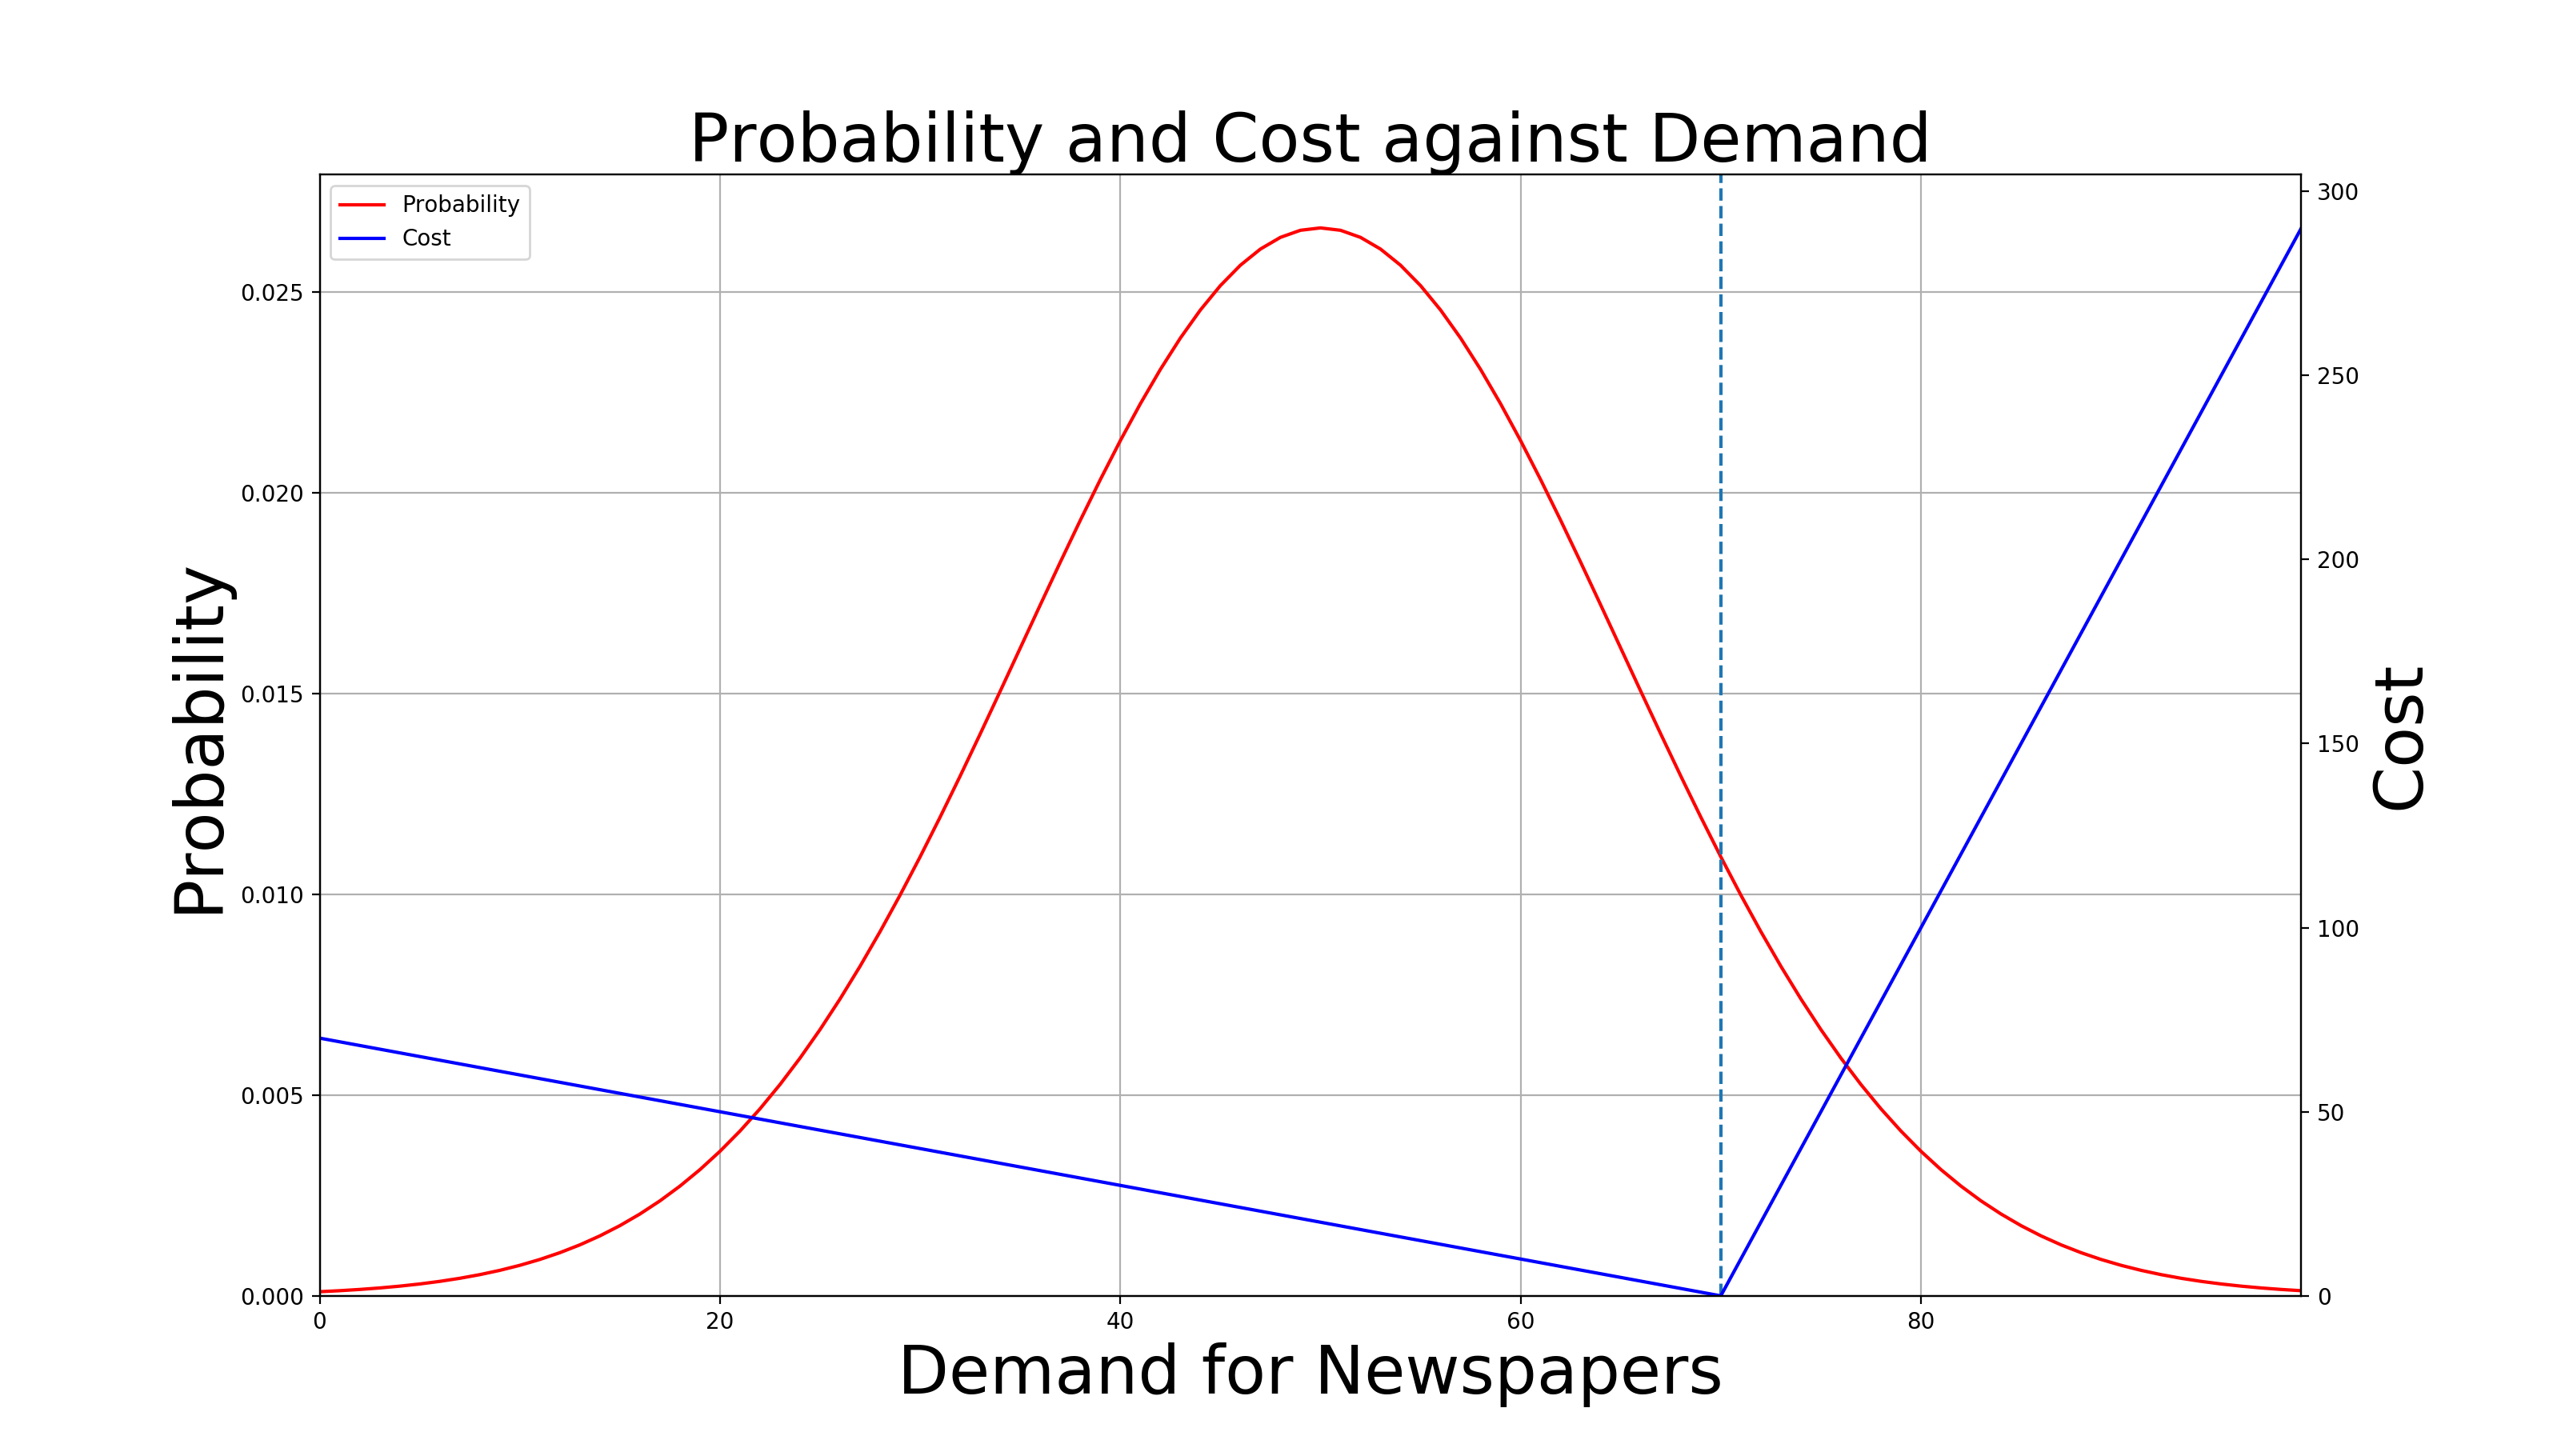
\includegraphics[width=12cm, height=8cm]{newsvendor.png}
\end{frame}

\begin{frame}
\frametitle{Solution to the Newsvendor problem}
\pause
\begin{itemize}[<+->]
\item For tractability, we assume newspapers are a continuous variable $x$
\item Then, we need to solve for the optimal supply $S$ that maximizes
$$g(S) = h \int_0^S (S-x) \cdot f(x) \cdot dx + p \int_S^{\infty} (x-S) \cdot f(x) \cdot dx$$
\item Setting $g'(S) =0$, we get:
$$\mbox{ Optimal Supply } S^* = F^{-1}(\frac p {p+h})$$
where $F(y) = \int_0^y f(x) dx$ is the CDF of daily demand
\item $\frac p {p+h}$ is known as the critical fractile
\item It is the fraction of days when the newsvendor goes ``out-of-stock''
\item Assuming the newsvendor always brings this optimal supply $S^*$
\item Solution details and connections with Financial Options Pricing \href{https://github.com/coverdrive/technical-documents/blob/master/supply_chain/NewsvendorOptionsPricing/NewsvendorOptionsPricing.pdf}{\underline{\textcolor{blue}{here}}}
\end{itemize}
\end{frame}

\begin{frame}
\frametitle{Multi-period: Single-store, Single-item Inventory Control}
\pause
\begin{itemize}[<+->]
\item The store experiences random daily demand given by PDF $f(x)$
\item The store can order daily from a supplier carrying infinite inventory
\item There's a cost associated with ordering, and order arrives in $L$ days
\item Like newsvendor, there's a Holding Cost $h$ and Stockout Cost $p$
\item This is an MDP where {\em State} is current Inventory Level at the store
\item {\em State} also includes current in-transit inventory (from supplier)
\item {\em Action} is quantity to order in any given {\em State}
\item {\em Reward} function has $h$, $p$ (just like newsvendor), and ordering cost
\item Transition probabilities are governed by demand distribution $f(x)$
\item This has a closed-form solution, similar to newsvendor fomula
\end{itemize}
\end{frame}

\begin{frame}
\frametitle{Optimal Ordering Policy (with Ordering Cost included)}
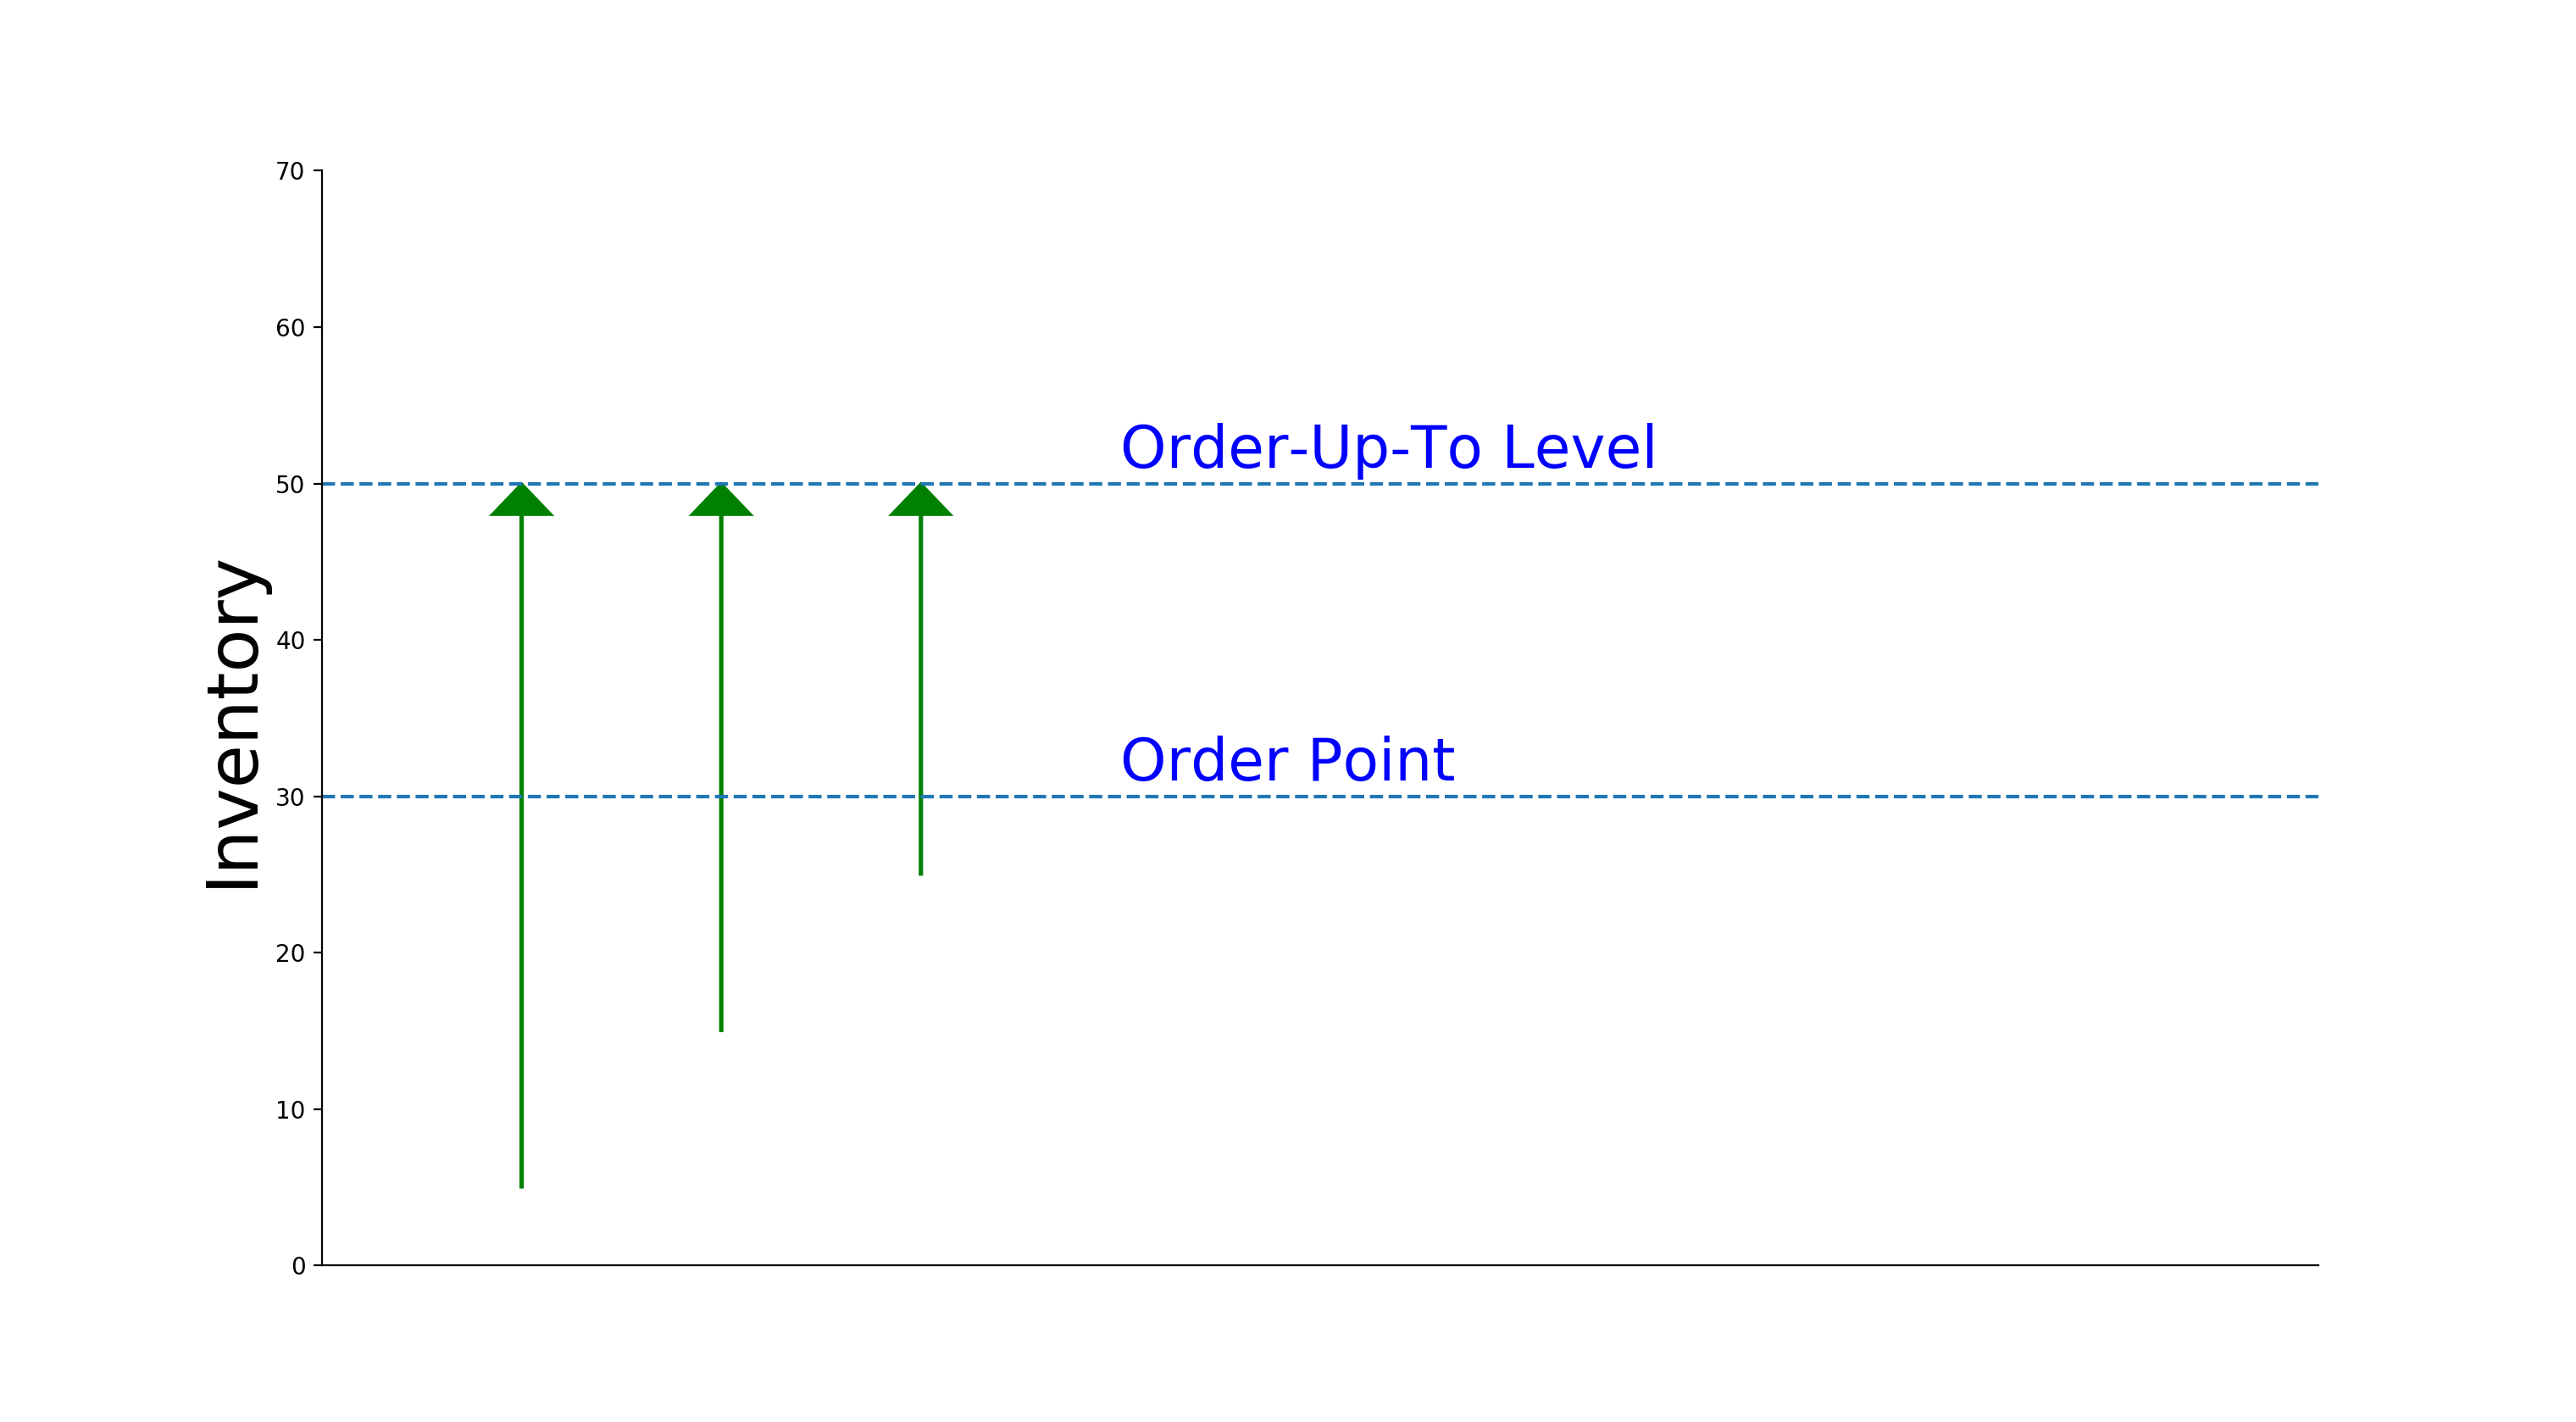
\includegraphics[width=12cm, height=8cm]{op_otl.png}
\end{frame}


\begin{frame}
\frametitle{The Core of Textbook Problem has this Pictorial Intuition}
\includegraphics[width=12cm, height=8cm]{newsvendor_arrow1.png}
\end{frame}


\begin{frame}
\frametitle{Costs viewed against End-of-Day Inventory}
\includegraphics[width=12cm, height=8cm]{newsvendor_arrow2.png}
\end{frame}

\begin{frame}
\frametitle{UnderCapacity and OverCapacity Costs}
\includegraphics[width=12cm, height=8cm]{capacity_costs.png}
\end{frame}

\begin{frame}
\frametitle{UnderCapacity Cost: Customer Psychology and Economics}
\pause
\begin{itemize}[<+->]
\item Retail Mantra: ``Stack it high and watch it fly''
\item Customers like to see shelves well stocked
\item Visual emptiness is known to be a sales deterrent
\item So, full-looking shelves are part of presentation strategy
\item At a certain level of emptiness, the deterrent rises sharply
\item Hence the convex nature of this cost curve
\item Note that this curve varies from item to item
\item It also varies from regular season to end of season
\item Modeling/calibrating this is tricky!
\item However, getting a basic model in place is vital
\end{itemize}
\end{frame}

\begin{frame}
\frametitle{OverCapacity Cost: Backroom Space Constraints}
\pause
\begin{itemize}[<+->]
\item Retail store backrooms have limited capacity
\item Typically tens of thousands of items compete for this space
\item Retailers like to have clean and organized backrooms
\item A perfect model is when all your inventory is on store shelves
\item With backroom used purely as a hub for home deliveries
\item Practically, some overflow from shelves is unavoidable
\item Hence, the convex nature of this curve
\item Modeling this is hard because it's a multi-item cost/constraint
\item Again, getting a basic model in place is vital
\end{itemize}
\end{frame}

\begin{frame}
\frametitle{What other costs are involved?}
\pause
\begin{itemize}[<+->]
\item Holding Cost: Interest on Inventory, Superficial Damage, Maintenance
\item Stockout Cost: Lost Sales, sometimes Lost Customers
\item Labor Cost: Replenishment involves movement from truck to shelf
\item Spoilage Cost: Food \& Beverages can have acute perishability
\item End-of-Season/Obsolescence Cost: Intersects with Clearance Pricing 
\end{itemize}
\end{frame}

\begin{frame}
\frametitle{Practical Inventory Control as a Markov Decision Process}
\pause
\begin{itemize}[<+->]
\item The store experiences random daily demand
\item The store can place a replenishment order in casepack mutiples
\item This is an MDP where {\em State} is current Inventory Level at the store
\item {\em State} also includes current in-transit inventory (from warehouse)
\item {\em Action} is the multiple of casepack to order (or not order)
\item {\em Reward} function involves all of the costs we went over earlier
\item State transitions governed by demand probability distribution
\item Solve: Dynamic Programming or Reinforcement Learning Algorithms
\end{itemize}
\end{frame}



\begin{frame}
\frametitle{Multi-node and Multi-item Inventory Control}
\pause
\begin{itemize}[<+->]
\item In practice, Inventory flows through a network of warehouses
\item From source (suppliers) to destination (stores or homes)
\item So, we have to solve a multi-``node'' Inventory Control problem
\item {\em State} is joint inventory across all nodes (and between nodes)
\item {\em Action} is recommended movements of inventory between nodes
\item {\em Reward} is the aggregate of daily costs across the network
\item In addition, we have multi-item constraints
\item Space and Throughput constraints are multi-item constraints
\item So, real-world problem is multi-node and multi-item (giant MDP)
\end{itemize}
\end{frame}

\begin{frame}
\frametitle{Clearance Pricing}
\pause
\begin{itemize}[<+->]
\item You are a few weeks away from end-of-season (eg: Christmas Trees)
\item Assume you have too much inventory in your store
\item What is the optimal sequence of price markdowns?
\item Under (uncertain) demand responding to markdowns
\item So as to maximize your total profit (sales revenue minus costs)
\item Note: There is a non-trivial cost of performing a markdown
\item If price markdowns are small, we end up with surplus at season-end
\item Surplus often needs to be disposed at poor salvage price
\item If price reductions are large, we run out of Christmas trees early
\item ``Stockout'' cost is considered to be large during holiday season
\end{itemize}
\end{frame}

\begin{frame}
\frametitle{MDP for Clearance Pricing}
\pause
\begin{itemize}
\item {\em State} is [Days Left, Current Inventory, Current Price, Market Info]
\item {\em Action} is Price Markdown
\item {\em Reward} includes Sales revenue, markdown cost, stockout cost, salvage
\item {\em Reward} \& {\em State}-transitions governed by {\em Price Elasticity of Demand}
\item Real-world {\em Model} can be quite complex (eg: competitor pricing)
\item Ambitious Idea: Blend Inventory and Price Control into one MDP
\end{itemize}
\end{frame}


\begin{frame}
\frametitle{Inputs to these MDPs (other than the costs)}
\pause
\begin{itemize}[<+->]
\item Daily Demand Forecast probability distribution function
\item Shelf Capacity
\item Casepack size
\item Lead Time (time from replenishment order to arrival on shelf)
\end{itemize}
\end{frame}

\begin{frame}
\frametitle{Where do these inputs come from?}
\pause
\begin{itemize}[<+->]
\item From solutions to various other Forecasting and Planning problems
\item Demand Forecasting is a statistical learning problem
\item Planning problems are Optimization problems
\item Some Planning Problems:
\begin{itemize}
\item Assortment Selection
\item Shelf-size Planning
\item Casepack Sizing
\item Network Planning (for Lead Time)
\item Labor Planning
\end{itemize}
\item Some of these planning problems based on Inventory Control solution
\item Chicken-and-egg issues resolvable by Simulations
\item Very important to design the interfaces consistently
\item Clean software framework for overall system design is vital to success
\end{itemize}
\end{frame}

\begin{frame}
\frametitle{Perspective from the Trenches (to solve MDPs)}
\pause
\begin{itemize}[<+->]
\item I always start with a simple version of problem to develop intuition
\item My first line of attack is DP customized to the problem structure
\item RL Algorithms that are my personal favorites (links to lectures):
\begin{itemize}
\item Deep Q-Network (DQN): Experience Replay, 2nd Target Network
\item \href{https://github.com/coverdrive/technical-documents/blob/master/finance/cme241/ValueFunctionGeometry.pdf}{\underline{\textcolor{blue}{Least Squares Policy Iteration (LSPI) - Batch Linear System}}}
\item \href {https://github.com/coverdrive/technical-documents/blob/master/finance/cme241/ValueFunctionGeometry.pdf}{\underline{\textcolor{blue}{Exact Gradient Temporal-Difference (GTD)}}}
\item \href{https://github.com/coverdrive/technical-documents/blob/master/finance/cme241/PolicyGradient.pdf}{\underline{\textcolor{blue}{Policy Gradient (esp. Natural Gradient, TRPO)}}}
\end{itemize}
\item Separate Model Estimation from Policy Optimization
\item So we could customize RL algorithms to take advantage of:
\begin{itemize}
\item Knowledge of transition probabilities
\item Knowledge of reward function
\item Any problem-specific structure that simplifies the algorithm
\end{itemize}
\item Feature Engineering based on known closed-form approximations
\item Many real-world, large-scale problems ultimately come down to
suitable choices of DNN architectures and hyperparameter tuning
\end{itemize}
\end{frame}



\end{document}
